\chapter{Mécanique lagrangienne}\label{ch:b3:lagrangian-mechanics}

Essayez d'écrire la loi de Newton pour un double pendule~: deux forces
de tension, dont aucune n'est connue à l'avance, changeant toutes deux
de direction à chaque instant, et quatre équations scalaires à démêler
rien que pour savoir comment évoluent deux angles. Faites de même pour
une perle sur un cerceau tournant, une chaîne de ressorts couplés, un
bras de robot. Les forces qui tiennent un système --- tiges, rails,
articulations --- ne travaillent pas, et pourtant la méthode de Newton
nous oblige à les traîner dans tout le calcul. Ce chapitre présente la
reformulation que Lagrange publia en 1788~: décrire le système par les
quelques coordonnées qui peuvent réellement varier, écrire une seule
fonction $L = E_k - E_p$, et une unique recette produit les équations
du mouvement dans n'importe quelles coordonnées, toutes tiges et tous
rails déjà éliminés. Mieux, la nouvelle formulation rend visible ce que
celle de Newton cache~: chaque symétrie de $L$ donne une grandeur
conservée --- la quantité de mouvement pour l'uniformité de l'espace,
l'énergie pour celle du temps ---, un résultat d'Emmy Noether devenu le
principe organisateur de la physique bien au-delà de la mécanique.

\section{Des forces aux coordonnées}

\begin{definition}[Contraintes, degrés de liberté, coordonnées généralisées]\label{def:b3:lagrangian-mechanics:coordinates}
\index{contrainte}\index{degrés de liberté}\index{coordonnées généralisées}
Une \emph{contrainte} est une condition géométrique imposée aux
positions d'un système --- une perle reste sur son fil, la tige d'un
pendule garde une longueur fixe, deux roues d'un même essieu tournent
ensemble. Une contrainte que l'on peut écrire comme une équation
$f(\vect r_1, \dots, \vect r_N, t) = 0$ entre les coordonnées (et
éventuellement le temps) est dite \emph{holonome}. Le nombre de façons
indépendantes dont la configuration peut encore varier est le nombre de
\emph{degrés de liberté} $n$~; tout jeu de $n$ grandeurs indépendantes
$q_1, \dots, q_n$ qui fixe complètement la configuration forme un jeu
de \emph{coordonnées généralisées} --- angles, longueurs ou tout
mélange commode. Leurs dérivées temporelles $\dot q_1, \dots, \dot q_n$
sont les \emph{vitesses généralisées}\index{vitesses généralisées}.
\end{definition}

\begin{example}[Compter les degrés de liberté]\label{ex:b3:lagrangian-mechanics:counting}
Un point sur une table~: $n = 2$. Un pendule plan de longueur fixe~: un
angle, $n = 1$. Un double pendule~: deux angles, $n = 1 + 1 = 2$. Une
perle sur un cerceau rigide~: un angle, $n = 1$ --- même si le cerceau
lui-même est forcé de tourner, car la rotation imposée n'ajoute aucune
liberté. Un solide libre dans l'espace~: trois coordonnées de son
centre plus trois angles, $n = 6$. Un gaz de $N$ molécules libres
(ponctuelles)~: $n = 3N$. Chaque \omterm{def:b3:lagrangian-mechanics:coordinates}{contrainte} holonome retire un degré de
liberté~: deux points reliés par une tige ont $3 + 3 - 1 = 5$.
\end{example}

\begin{omfigure}
\begin{tikzpicture}[font=\small, >=Stealth]
  % (a) plane pendulum
  \begin{scope}
    \draw[thick] (-1,0) -- (1,0);
    \foreach \i in {-0.8,-0.5,-0.2,0.1,0.4,0.7} \draw (\i,0) -- (\i+0.18,0.16);
    \fill (0,0) circle (1.5pt);
    \draw[dashed] (0,0) -- (0,-2.2);
    \draw[thick] (0,0) -- (-55:2.1);
    \fill[omDef] (-55:2.1) circle (3pt);
    \draw[->] (0,-1.0) arc (-90:-55:1.0);
    \node at (-72:1.35) {$\theta$};
    \node at (-55:2.5) {$m$};
    \node at ($(-55:1.35)+(0.28,0.12)$) {$\ell$};
    \node at (0,-2.9) {une coordonnée~: $\theta$};
  \end{scope}
  % (b) bead on rotating hoop
  \begin{scope}[xshift=6.2cm]
    \coordinate (C) at (0,-2.35);
    \draw[thick] (C) circle (1.55);
    \draw[dashed] (0,-0.3) -- (0,-4.6);
    \draw[->, thick] (0.35,-0.15) arc (20:160:0.37);
    \node at (0,0.25) {$\omega$};
    \fill (C) circle (1pt);
    \draw (C) -- ++(-50:1.55);
    \fill[omDef] ($(C)+(-50:1.55)$) circle (3pt);
    \draw[->] ($(C)+(0,-0.85)$) arc (-90:-50:0.85);
    \node at ($(C)+(-70:1.18)$) {$\theta$};
    \node at ($(C)+(-38:2.0)$) {$m$};
    \draw (C) -- ++(135:1.55);
    \node at (-1.35,-1.35) {$R$};
    \node at (0,-4.95) {une coordonnée~: $\theta$};
  \end{scope}
  % (c) double pendulum
  \begin{scope}[xshift=11.4cm]
    \draw[thick] (-0.9,0) -- (0.9,0);
    \foreach \i in {-0.7,-0.4,-0.1,0.2,0.5} \draw (\i,0) -- (\i+0.18,0.16);
    \fill (0,0) circle (1.5pt);
    \draw[dashed] (0,0) -- (0,-1.7);
    \draw[thick] (0,0) -- (-65:1.5) coordinate (m1);
    \fill[omDef] (m1) circle (2.6pt);
    \draw[dashed] (m1) -- ++(0,-1.5);
    \draw[thick] (m1) -- ++(-40:1.5) coordinate (m2);
    \fill[omThm] (m2) circle (2.6pt);
    \draw[->] (0,-0.8) arc (-90:-65:0.8);
    \node at (-80:1.1) {$\theta_1$};
    \draw[->] ($(m1)+(0,-0.75)$) arc (-90:-40:0.75);
    \node at ($(m1)+(-68:1.05)$) {$\theta_2$};
    \node at (0.3,-3.4) {deux coordonnées~: $\theta_1, \theta_2$};
  \end{scope}
\end{tikzpicture}

{\small \omterm{def:b3:lagrangian-mechanics:coordinates}{Coordonnées généralisées}~: chaque système est décrit par les
angles qui peuvent réellement varier, non par les coordonnées
cartésiennes de ses masses. Les tensions des tiges et la réaction
normale du cerceau n'apparaissent jamais.}
\end{omfigure}

\section{Le principe de moindre action}

\begin{definition}[Lagrangien et action]\label{def:b3:lagrangian-mechanics:action}
\index{lagrangien}\index{action}
Le \emph{lagrangien} d'un système mécanique dont les forces dérivent
d'une énergie potentielle $E_p$ est la fonction des coordonnées, des
vitesses et éventuellement du temps
\[
L(q, \dot q, t) = E_k - E_p ,
\]
énergie cinétique \emph{moins} énergie potentielle, toutes deux
exprimées dans les \omterm{def:b3:lagrangian-mechanics:coordinates}{coordonnées généralisées}. L'\emph{action} d'un
mouvement concevable $q(t)$ entre les extrémités fixées $q(t_1)$ et
$q(t_2)$ est le nombre
\[
S[q] = \int_{t_1}^{t_2} L\big(q(t), \dot q(t), t\big)\,\dd t .
\]
$S$ est une \emph{fonctionnelle}~: elle avale un chemin entier et
renvoie un seul nombre, en joule-secondes --- l'unité de la constante
de Planck.
\end{definition}

\begin{theorem}[Principe de Hamilton et équations d'Euler--Lagrange]\label{thm:b3:lagrangian-mechanics:euler-lagrange}
\index{principe de Hamilton}\index{équations d'Euler--Lagrange}\index{moindre action}
Parmi tous les mouvements concevables joignant les deux mêmes
extrémités dans le même temps, le mouvement réel est celui qui rend
l'\omterm{def:b3:lagrangian-mechanics:action}{action} \emph{stationnaire} (\emph{\omterm{thm:b3:lagrangian-mechanics:euler-lagrange}{principe de Hamilton}}, ou principe
de \emph{\omterm{thm:b3:lagrangian-mechanics:euler-lagrange}{moindre action}}). De façon équivalente, le mouvement obéit aux
\emph{\omterm{thm:b3:lagrangian-mechanics:euler-lagrange}{équations d'Euler--Lagrange}}
\[
\frac{\dd}{\dd t}\frac{\partial L}{\partial\dot q_i}
 - \frac{\partial L}{\partial q_i} = 0 ,
\qquad i = 1, \dots, n :
\]
une équation du second ordre par degré de liberté, quelles que soient
les coordonnées choisies.
\end{theorem}

\begin{proof}
Déformons le chemin~: $q_i(t) \to q_i(t) + \delta q_i(t)$ avec
$\delta q_i(t_1) = \delta q_i(t_2) = 0$. Au premier ordre,
\[
\delta S = \int_{t_1}^{t_2}\sum_i\Big(
  \frac{\partial L}{\partial q_i}\,\delta q_i
 + \frac{\partial L}{\partial\dot q_i}\,\delta\dot q_i\Big)\dd t
 = \int_{t_1}^{t_2}\sum_i\Big(
  \frac{\partial L}{\partial q_i}
 - \frac{\dd}{\dd t}\frac{\partial L}{\partial\dot q_i}\Big)\delta q_i\,\dd t ,
\]
après intégration par parties du second terme ($\delta\dot q_i =
\dd(\delta q_i)/\dd t$) et suppression du terme de bord, qui s'annule
aux extrémités fixées. Si $\delta S = 0$ pour \emph{toute} déformation,
la parenthèse doit s'annuler à chaque instant et pour chaque $i$ ---
si elle était positive quelque part, une bosse $\delta q_i$ concentrée
là donnerait $\delta S \neq 0$. La réciproque se lit sur la même ligne.
\end{proof}

\begin{omfigure}
\begin{tikzpicture}[font=\small, >=Stealth]
  \draw[->] (0,0) -- (7.6,0) node[right] {$t$};
  \draw[->] (0,0) -- (0,3.4) node[above] {$q$};
  \fill (0.8,0.7) circle (2pt) node[below left] {$q(t_1)$};
  \fill (6.8,2.3) circle (2pt) node[above right] {$q(t_2)$};
  \draw[omDef, very thick] (0.8,0.7) .. controls (2.6,2.6) and (5.0,1.4) .. (6.8,2.3);
  \draw[omExo, dashed] (0.8,0.7) .. controls (2.2,0.6) and (5.4,0.9) .. (6.8,2.3);
  \draw[omExo, dashed] (0.8,0.7) .. controls (3.0,3.6) and (5.2,2.9) .. (6.8,2.3);
  \node[omDef] at (1.9,3.35) {chemin réel};
  \draw[->, omDef] (2.25,3.15) -- (2.85,2.3);
  \node[omExo] at (3.4,0.42) {chemins variés};
  \draw[<->] (4.1,1.62) -- (4.1,2.62);
  \node at (4.55,2.15) {$\delta q$};
\end{tikzpicture}

{\small Le \omterm{thm:b3:lagrangian-mechanics:euler-lagrange}{principe de Hamilton}~: parmi tous les chemins de mêmes
extrémités et de même durée, le chemin réel rend $S = \int L\,\dd t$
stationnaire --- les déformations $\delta q$ au premier ordre ne
changent $S$ qu'au second ordre.}
\end{omfigure}

\begin{proposition}[Newton retrouvé]\label{prop:b3:lagrangian-mechanics:newton}
Pour une particule en coordonnées cartésiennes, $L = \tfrac12 m(\dot x^2 +
\dot y^2 + \dot z^2) - E_p(x,y,z)$, et les \omterm{thm:b3:lagrangian-mechanics:euler-lagrange}{équations d'Euler--Lagrange}
s'écrivent $m\ddot x = -\partial E_p/\partial x$, de même pour $y$ et $z$~:
exactement $m\vect a = \vect F$. Mécaniques lagrangienne et newtonienne
s'accordent partout où les deux s'appliquent~; la forme nouvelle survit
simplement à un changement de coordonnées, ce que ne font pas les
équations en composantes de Newton.
\end{proposition}

\begin{proof}
$\partial L/\partial\dot x = m\dot x$, $\partial L/\partial x =
-\partial E_p/\partial x$~; l'équation d'Euler--Lagrange est
$\dd(m\dot x)/\dd t + \partial E_p/\partial x = 0$.
\end{proof}

\begin{remark}[Pourquoi les forces de liaison disparaissent]\label{rem:b3:lagrangian-mechanics:constraints}
La tension d'une tige, la réaction normale d'un rail, agissent
perpendiculairement à tout déplacement que la \omterm{def:b3:lagrangian-mechanics:coordinates}{contrainte} autorise~:
elles ne travaillent dans aucun mouvement compatible avec la
\omterm{def:b3:lagrangian-mechanics:coordinates}{contrainte}. Comme l'\omterm{def:b3:lagrangian-mechanics:action}{action} est bâtie sur des énergies évaluées
uniquement le long de tels mouvements, ces forces n'entrent jamais dans
$L$ --- c'est là le miracle pratique de la méthode. La justification
générale (le principe des travaux virtuels de d'Alembert) est admise
ici~; pour chaque système de ce livre, la recette ci-dessous se vérifie
directement contre Newton, comme l'a amorcé
\cref{prop:b3:lagrangian-mechanics:newton}. Si l'on veut la force de
liaison elle-même --- la tige va-t-elle casser~? ---, on revient à
Newton pour cette seule force, le mouvement étant déjà connu.
\end{remark}

\begin{method}[La recette lagrangienne]\label{met:b3:lagrangian-mechanics:recipe}
(1) Compter les \omterm{def:b3:lagrangian-mechanics:coordinates}{degrés de liberté} et choisir les coordonnées $q_i$ ---
angles pour les rotations, abscisses le long des rails. (2) Exprimer
les positions $\vect r(q_i, t)$, dériver pour obtenir les vitesses et
écrire $E_k$~; écrire $E_p$. (3) $L = E_k - E_p$, en laissant tomber
toute constante additive. (4) Une équation d'Euler--Lagrange par
coordonnée. (5) Avant de résoudre, récolter les grandeurs conservées~:
\omterm{def:b3:lagrangian-mechanics:momentum}{coordonnées cycliques} (\cref{def:b3:lagrangian-mechanics:momentum}) et
\omterm{prop:b3:lagrangian-mechanics:energy}{fonction énergie} (\cref{prop:b3:lagrangian-mechanics:energy}). (6)
Vérifier les cas limites~: petits angles, rotation coupée, cas
particuliers connus.
\end{method}

\begin{example}[Le pendule, en trois lignes]\label{ex:b3:lagrangian-mechanics:pendulum}
Une seule coordonnée $\theta$~; $\vect v = \ell\dot\theta\,\vect e_\theta$,
donc $E_k = \tfrac12 m\ell^2\dot\theta^2$ et $E_p = -mg\ell\cos\theta$.
Alors $L = \tfrac12 m\ell^2\dot\theta^2 + mg\ell\cos\theta$, et
$\dd(m\ell^2\dot\theta)/\dd t = -mg\ell\sin\theta$~:
\[
\ddot\theta = -\frac{g}{\ell}\sin\theta ,
\]
l'équation que le volume de première année tirait du moment du poids
--- sans jamais mentionner la tension.
\end{example}

\begin{example}[Perle sur un cerceau tournant]\label{ex:b3:lagrangian-mechanics:hoop}
Une perle de masse $m$ glisse sur un cerceau circulaire vertical de
rayon $R$ forcé de tourner autour de son diamètre vertical à $\omega$
constante (\cref{ex:b3:lagrangian-mechanics:counting}). Une seule
coordonnée, l'angle polaire $\theta$ compté depuis le bas. La vitesse
de la perle a une composante $R\dot\theta$ le long du cerceau et une
composante $\omega R\sin\theta$ due à la rotation imposée, qui lui est
perpendiculaire~:
\[
L = \tfrac12 mR^2\dot\theta^2 + \tfrac12 m\omega^2R^2\sin^2\theta
 + mgR\cos\theta ,
\qquad
mR^2\ddot\theta = m\omega^2R^2\sin\theta\cos\theta - mgR\sin\theta .
\]
Les équilibres où $\ddot\theta = 0$~: le bas $\theta = 0$ (et le haut,
toujours instable) et, lorsque $\omega^2 > g/R$, une nouvelle paire
$\cos\theta_{\text{eq}} = g/\omega^2R$. Écrivez l'équation sous la forme
$mR^2\ddot\theta = -\dd U_{\text{eff}}/\dd\theta$ avec
l'\emph{énergie potentielle effective}\index{énergie potentielle effective}
\[
U_{\text{eff}}(\theta) = -mgR\cos\theta
 - \tfrac12 m\omega^2R^2\sin^2\theta
\]
rend la géométrie visible~: en dessous de la vitesse critique
$\omega_{\text{c}} = \sqrt{g/R}$ le bas est un puits~; au-dessus, le
bas devient un sommet et la perle se stabilise sur le flanc, d'autant
plus haut que le cerceau tourne vite --- le principe du régulateur à
boules qui gouvernait les machines à vapeur.
\end{example}

\begin{omfigure}
\begin{tikzpicture}
  \begin{axis}[omaxis, axis x line=bottom, axis y line=left,
    width=11.4cm, height=5.6cm, xmin=-180, xmax=180,
    ymin=-1.65, ymax=1.2, xlabel={$\theta$ (degrés)},
    xlabel style={at={(axis description cs:0.5,-0.1)}, anchor=north},
    ylabel={$U_{\text{eff}}/mgR$}, xtick={-180,-90,0,90,180}, ytick=\empty,
    clip=false,
    legend style={font=\scriptsize, at={(0.5,-0.32)}, anchor=north,
      draw=none, fill=none, legend columns=2}]
    \addplot[omDef, thick, domain=-180:180, samples=90]
      {-cos(x) - 0.25*sin(x)^2};
    \addlegendentry{$\omega^2 = g/2R$ (lent)~: puits en $\theta = 0$}
    \addplot[omThm, thick, domain=-180:180, samples=90]
      {-cos(x) - 1.0*sin(x)^2};
    \addlegendentry{$\omega^2 = 2g/R$ (rapide)~: puits à $\pm 60^\circ$}
    \fill[omThm] (axis cs:60,-1.25) circle (1.8pt);
    \fill[omThm] (axis cs:-60,-1.25) circle (1.8pt);
    \fill[omDef] (axis cs:0,-1) circle (1.8pt);
  \end{axis}
\end{tikzpicture}

{\small Le potentiel effectif de la perle sur le cerceau tournant.
Lorsque $\omega$ franchit $\sqrt{g/R}$, l'unique puits du bas se scinde
en deux puits symétriques~: l'angle d'équilibre croît avec la vitesse
de rotation.}
\end{omfigure}

\section{Symétries et lois de conservation}

\begin{definition}[Moment conjugué, coordonnée cyclique]\label{def:b3:lagrangian-mechanics:momentum}
\index{moment conjugué}\index{coordonnée cyclique}
Le \emph{moment conjugué} de la coordonnée $q_i$ est
\[
p_i = \frac{\partial L}{\partial\dot q_i} .
\]
Pour une coordonnée cartésienne, c'est la quantité de mouvement
ordinaire $m\dot x$~; pour un angle, c'est un moment cinétique. Une
coordonnée qui ne figure pas dans $L$ (alors que sa vitesse y figure)
est dite \emph{cyclique}.
\end{definition}

\begin{proposition}[Les coordonnées cycliques donnent des lois de conservation]\label{prop:b3:lagrangian-mechanics:cyclic}
Si $q_i$ est cyclique, son \omterm{def:b3:lagrangian-mechanics:momentum}{moment conjugué} est conservé~:
$\partial L/\partial q_i = 0$ entraîne $\dd p_i/\dd t = 0$. Choisir les
coordonnées de façon qu'un maximum d'entre elles soient cycliques est
l'étape la plus efficace de la résolution d'un problème de mécanique.
\end{proposition}

\begin{proof}
Immédiat, par l'équation d'Euler--Lagrange relative à $q_i$.
\end{proof}

\begin{example}[Force centrale, résolue à vue]\label{ex:b3:lagrangian-mechanics:central}
Une particule dans un potentiel central $E_p(r)$, en coordonnées
polaires dans son plan de mouvement~:
\[
L = \tfrac12 m(\dot r^2 + r^2\dot\varphi^2) - E_p(r) .
\]
$\varphi$ est cyclique, donc $p_\varphi = mr^2\dot\varphi$ --- le
moment cinétique --- est conservé~: la loi des aires de Kepler, que le
volume de première année tirait de l'équation du moment cinétique,
tombe ici avant même qu'aucune équation ne soit résolue. L'équation
radiale restante est $m\ddot r = mr\dot\varphi^2 - E_p'(r)$,
c'est-à-dire le mouvement à une dimension dans le potentiel effectif
$E_p(r) + p_\varphi^2/2mr^2$ de ce volume.
\end{example}

\begin{theorem}[Théorème de Noether]\label{thm:b3:lagrangian-mechanics:noether}
\index{théorème de Noether}\index{symétrie}
À toute symétrie continue du \omterm{def:b3:lagrangian-mechanics:action}{lagrangien} correspond une grandeur
conservée. Précisément~: si le décalage $q_i \to q_i + \varepsilon\,K_i(q)$
laisse $L$ inchangé au premier ordre en $\varepsilon$ pour tous les
mouvements, alors
\[
Q = \sum_i p_i\,K_i(q)
\]
est constante le long de tout mouvement réel. L'uniformité de l'espace
(invariance par translation) donne la quantité de mouvement~;
l'isotropie de l'espace (invariance par rotation) donne le moment
cinétique~; l'uniformité du temps donne l'énergie
(\cref{prop:b3:lagrangian-mechanics:energy}).
\end{theorem}

\begin{proof}
L'invariance au premier ordre signifie
$0 = \delta L = \sum_i\big(\partial_{q_i}L\,K_i +
\partial_{\dot q_i}L\,\dot K_i\big)\varepsilon$. Sur un mouvement réel,
$\partial_{q_i}L = \dot p_i$ par Euler--Lagrange, si bien que la
parenthèse vaut $\sum_i(\dot p_iK_i + p_i\dot K_i) = \dd Q/\dd t$. Une
\omterm{def:b3:lagrangian-mechanics:momentum}{coordonnée cyclique} est le cas particulier $K_i = \delta_{ij}$. Le cas
de la translation du temps demande le calcul distinct de
\cref{prop:b3:lagrangian-mechanics:energy}~; le théorème complet, pour
des transformations qui changent aussi $t$ ou modifient $L$ d'une
dérivée totale, se démontre dans les cours de mécanique analytique et
est admis ici dans cette généralité.
\end{proof}

\begin{proposition}[La fonction énergie]\label{prop:b3:lagrangian-mechanics:energy}
\index{fonction énergie}
Le long de tout mouvement, la \emph{\omterm{prop:b3:lagrangian-mechanics:energy}{fonction énergie}}
\[
h = \sum_i \dot q_i\,\frac{\partial L}{\partial\dot q_i} - L
\qquad\text{obéit à}\qquad
\frac{\dd h}{\dd t} = -\frac{\partial L}{\partial t} .
\]
Si $L$ ne dépend pas explicitement du temps, $h$ est conservée. Si de
plus les relations $\vect r(q)$ entre positions et coordonnées ne font
pas intervenir le temps --- pas de rotation imposée, pas de support
mobile ---, alors $E_k$ est une forme quadratique des $\dot q_i$ et
$h = E_k + E_p$~: l'énergie mécanique. Avec une \omterm{def:b3:lagrangian-mechanics:coordinates}{contrainte} dépendant du
temps, $h$ est encore conservée dès que $\partial L/\partial t = 0$,
mais ce n'est \emph{pas} l'énergie~: le moteur qui impose la \omterm{def:b3:lagrangian-mechanics:coordinates}{contrainte}
échange du travail avec le système.
\end{proposition}

\begin{proof}
$\dd h/\dd t = \sum_i(\ddot q_ip_i + \dot q_i\dot p_i) -
\sum_i(\partial_{q_i}L\,\dot q_i + \partial_{\dot q_i}L\,\ddot q_i) -
\partial_tL$. Les termes en $\ddot q_i$ se compensent~; les \omterm{thm:b3:lagrangian-mechanics:euler-lagrange}{équations
d'Euler--Lagrange} transforment $\dot p_i$ en $\partial_{q_i}L$, ce qui
annule la paire suivante~; il reste $-\partial_tL$. Si $E_k = \tfrac12\sum a_{jk}(q)\dot
q_j\dot q_k$, l'identité d'Euler donne $\sum\dot
q_i\,\partial E_k/\partial\dot q_i = 2E_k$, donc $h = 2E_k - (E_k - E_p)
= E_k + E_p$.
\end{proof}

\begin{example}[Le cerceau tournant conserve $h$, non $E$]\label{ex:b3:lagrangian-mechanics:hoop-energy}
Pour la perle de \cref{ex:b3:lagrangian-mechanics:hoop}, $L$ ne contient
pas $t$ explicitement, donc $h = \tfrac12 mR^2\dot\theta^2 + U_{\text{eff}}
(\theta)$ est conservée --- mais l'énergie mécanique $E = \tfrac12
mR^2\dot\theta^2 + \tfrac12 m\omega^2R^2\sin^2\theta - mgR\cos\theta$
ne l'est pas~: $E = h + m\omega^2R^2\sin^2\theta$ varie à mesure que la
perle glisse. L'écart est le travail du moteur qui maintient $\omega$
constante pendant que la distance de la perle à l'axe change.
\end{example}

\section{Particules chargées et petites oscillations}

\begin{proposition}[Lagrangien d'une particule chargée]\label{prop:b3:lagrangian-mechanics:charge}
\index{potentiel dépendant de la vitesse}
Dans un champ électromagnétique décrit par les potentiels $V$ et
$\vect A$ (avec $\vect E = -\vect\nabla V - \partial_t\vect A$ et
$\vect B = \operatorname{\vect{curl}}\vect A$, comme au volume de
deuxième année), le \omterm{def:b3:lagrangian-mechanics:action}{lagrangien}
\[
L = \tfrac12 m\vect v^{\,2} - qV + q\,\vect v\cdot\vect A
\]
donne, par les \omterm{thm:b3:lagrangian-mechanics:euler-lagrange}{équations d'Euler--Lagrange}, exactement la force de
Lorentz $m\dot{\vect v} = q(\vect E + \vect v\wedge\vect B)$. La force
magnétique, qui ne travaille pas et ne dérive d'aucune énergie
potentielle ordinaire, entre par un terme linéaire en la vitesse~; le
\omterm{def:b3:lagrangian-mechanics:momentum}{moment conjugué} devient $\vect p = m\vect v + q\vect A$, et non plus
$m\vect v$ seul.
\end{proposition}

\begin{proof}
Pour la composante $x$~: $p_x = m\dot x + qA_x$, et
$\partial_xL = -q\,\partial_xV + q\,\vect v\cdot\partial_x\vect A$.
L'équation d'Euler--Lagrange donne $m\ddot x = -q\,\partial_xV -
q\,\dd A_x/\dd t + q\,\vect v\cdot\partial_x\vect A$. Le long du
mouvement $\dd A_x/\dd t = \partial_tA_x + (\vect v\cdot\vect\nabla)A_x$,
donc $m\ddot x = qE_x + q\big[\vect v\cdot\partial_x\vect A - (\vect v\cdot
\vect\nabla)A_x\big]$, et la parenthèse est la composante $x$ de $\vect
v\wedge(\vect\nabla\wedge\vect A) = \vect v\wedge\vect B$ --- il suffit
de développer les deux pour le vérifier.
\end{proof}

\begin{proposition}[Petites oscillations et modes propres]\label{prop:b3:lagrangian-mechanics:modes}
\index{modes propres}\index{petites oscillations}
Au voisinage d'un équilibre stable $q^{\text{eq}}$, développons $L$ au
second ordre en les écarts $u_i = q_i - q_i^{\text{eq}}$~:
$L \approx \tfrac12\sum m_{ij}\dot u_i\dot u_j -
\tfrac12\sum k_{ij}u_iu_j$ avec des matrices symétriques constantes. Les
équations du mouvement sont linéaires, et tout mouvement est une
superposition de \emph{\omterm{prop:b3:lagrangian-mechanics:modes}{modes propres}}~: oscillations collectives $u_i(t) = a_i\cos(\Omega t
+ \phi)$ où toutes les coordonnées vibrent à une même fréquence, les
amplitudes et les fréquences résolvant $\sum_j(k_{ij} -
\Omega^2m_{ij})\,a_j = 0$ --- un problème matriciel aux valeurs
propres, avec $n$ modes pour $n$ \omterm{def:b3:lagrangian-mechanics:coordinates}{degrés de liberté}.
\end{proposition}

\begin{proof}
Les termes linéaires s'annulent à un équilibre~; les \omterm{thm:b3:lagrangian-mechanics:euler-lagrange}{équations
d'Euler--Lagrange} du $L$ quadratique s'écrivent
$\sum_jm_{ij}\ddot u_j = -\sum_jk_{ij}u_j$. En y injectant
l'oscillation d'essai, on obtient le système linéaire annoncé, qui n'a
un vecteur d'amplitudes non nul que si $\det(k_{ij} -
\Omega^2m_{ij}) = 0$~: $n$ valeurs de $\Omega^2$, toutes positives à un
équilibre stable. Que le mouvement général soit une superposition des
modes est la diagonalisation simultanée de deux formes quadratiques, un
résultat de l'algèbre linéaire du volume de mathématiques de deuxième
année~; la complétude est admise.
\end{proof}

\begin{example}[Deux pendules couplés par un ressort]\label{ex:b3:lagrangian-mechanics:coupled}
Deux pendules identiques (masse $m$, longueur $\ell$), leurs masses
reliées par un ressort de raideur $k$ détendu quand les deux pendent à
la verticale. Pour de petits angles,
\[
L = \tfrac12 m\ell^2(\dot\theta_1^2 + \dot\theta_2^2)
 - \tfrac12 mg\ell(\theta_1^2 + \theta_2^2)
 - \tfrac12 k\ell^2(\theta_2 - \theta_1)^2 .
\]
La symétrie suggère les combinaisons $s = \theta_1 + \theta_2$ et $d =
\theta_1 - \theta_2$, qui découplent les équations~: le \emph{mode en
phase} ($\theta_1 = \theta_2$, ressort inerte) à $\Omega_1 =
\sqrt{g/\ell}$, et le \emph{mode en opposition} ($\theta_1 = -\theta_2$,
ressort deux fois plus étiré) à $\Omega_2 = \sqrt{g/\ell + 2k/m}$.
Lancez un seul pendule --- un mélange égal des deux modes --- et
l'énergie migre entièrement d'un pendule à l'autre puis revient, à la
fréquence de battement $(\Omega_2 - \Omega_1)/2\pi$~: la démonstration
des pendules couplés, et le mécanisme de tout transfert résonnant
d'énergie, des circuits accordés aux vibrations moléculaires.
\end{example}

\begin{omfigure}
\begin{tikzpicture}[font=\small, >=Stealth]
  % in-phase mode
  \begin{scope}
    \draw[thick] (-0.4,0) -- (3.4,0);
    \foreach \i in {-0.2,0.3,0.8,1.3,1.8,2.3,2.8} \draw (\i,0) -- (\i+0.18,0.16);
    \fill (0.5,0) circle (1.2pt);
    \fill (2.5,0) circle (1.2pt);
    \draw[thick] (0.5,0) -- ++(-75:1.9) coordinate (a1);
    \draw[thick] (2.5,0) -- ++(-75:1.9) coordinate (a2);
    \fill[omDef] (a1) circle (2.6pt);
    \fill[omDef] (a2) circle (2.6pt);
    \draw[decorate, decoration={coil, aspect=0.6, segment length=3pt, amplitude=2pt}] (a1) -- (a2);
    \draw[->, omDef] ($(a1)+(0.05,-0.3)$) -- ++(0.5,0);
    \draw[->, omDef] ($(a2)+(0.05,-0.3)$) -- ++(0.5,0);
    \node at (1.5,-2.9) {en phase~: $\Omega_1 = \sqrt{g/\ell}$};
  \end{scope}
  % opposed mode
  \begin{scope}[xshift=6.4cm]
    \draw[thick] (-0.4,0) -- (3.4,0);
    \foreach \i in {-0.2,0.3,0.8,1.3,1.8,2.3,2.8} \draw (\i,0) -- (\i+0.18,0.16);
    \fill (0.5,0) circle (1.2pt);
    \fill (2.5,0) circle (1.2pt);
    \draw[thick] (0.5,0) -- ++(-105:1.9) coordinate (b1);
    \draw[thick] (2.5,0) -- ++(-75:1.9) coordinate (b2);
    \fill[omThm] (b1) circle (2.6pt);
    \fill[omThm] (b2) circle (2.6pt);
    \draw[decorate, decoration={coil, aspect=0.6, segment length=5pt, amplitude=2pt}] (b1) -- (b2);
    \draw[->, omThm] ($(b1)+(-0.05,-0.3)$) -- ++(-0.5,0);
    \draw[->, omThm] ($(b2)+(0.05,-0.3)$) -- ++(0.5,0);
    \node at (1.5,-2.9) {en opposition~: $\Omega_2 = \sqrt{g/\ell + 2k/m}$};
  \end{scope}
\end{tikzpicture}

{\small Les deux \omterm{prop:b3:lagrangian-mechanics:modes}{modes propres} des pendules couplés. En phase, le
ressort ne s'étire jamais et la fréquence est celle du pendule libre~;
en opposition, chaque masse ressent le ressort doublé.}
\end{omfigure}

\begin{omfigure}
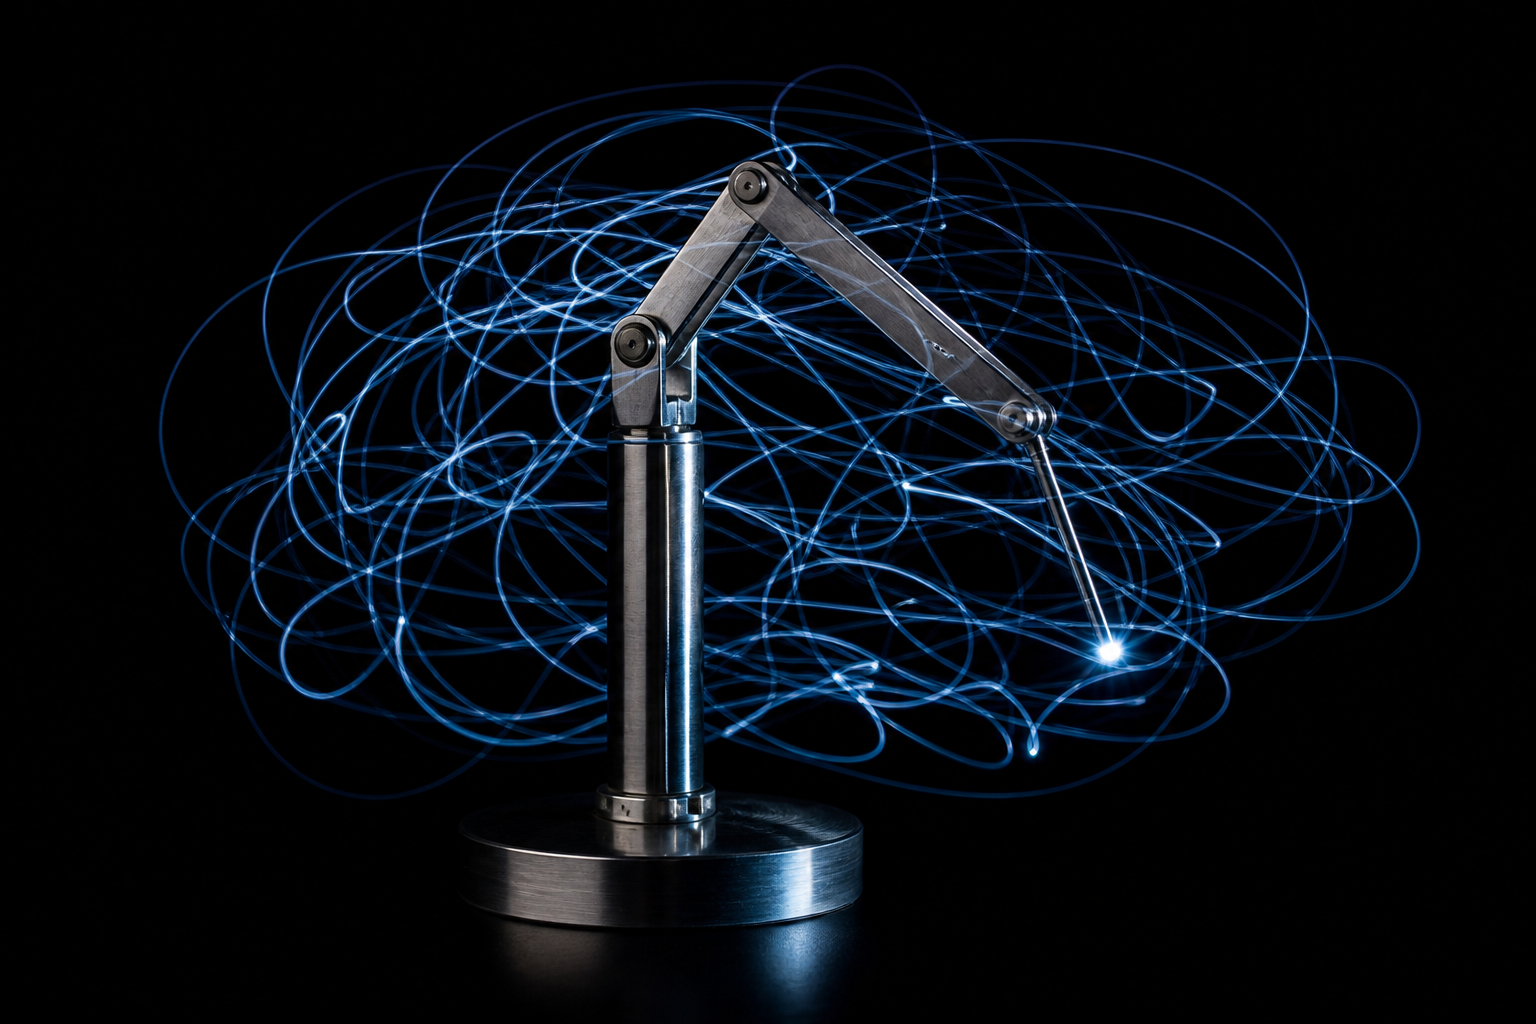
\includegraphics[width=0.58\linewidth]{images/book5/ai/b5-01-double-pendulum-trace.png}

{\small Un double pendule photographié en pose longue~: deux coordonnées, un seul \omterm{def:b3:lagrangian-mechanics:action}{lagrangien}, et un mouvement qu'aucune formule ne prédit longtemps --- la machinerie de \omterm{thm:b3:lagrangian-mechanics:euler-lagrange}{moindre action} de ce chapitre écrit les équations~; le chaos rend leurs solutions modestes.}
\end{omfigure}

\section{Exercices}

\begin{exercise}[$\star$]\label{exo:b3:lagrangian-mechanics:1}
Compter les \omterm{def:b3:lagrangian-mechanics:coordinates}{degrés de liberté} et proposer des \omterm{def:b3:lagrangian-mechanics:coordinates}{coordonnées
généralisées}~: (a) une particule à l'intérieur d'un bol fixe~; (b) un
cylindre roulant sans glisser sur un plan incliné fixe~; (c) un double
pendule dont le pivot supérieur coulisse sur un rail horizontal~; (d)
un haltère (deux masses, tige rigide) dans l'espace~; (e) deux perles
sur un même fil circulaire fixe. Laquelle de ces \omterm{def:b3:lagrangian-mechanics:coordinates}{contraintes} relie des
vitesses plutôt que des positions, et pourquoi est-elle néanmoins
intégrable en une \omterm{def:b3:lagrangian-mechanics:coordinates}{contrainte} holonome~?
\end{exercise}

\begin{exercise}[$\star$]\label{exo:b3:lagrangian-mechanics:2}
Pour le pendule plan (\cref{ex:b3:lagrangian-mechanics:pendulum})~:
(a) vérifier les dimensions de $L$ et de $p_\theta =
\partial L/\partial\dot\theta$~; (b) identifier physiquement
$p_\theta$~; (c) obtenir la période aux petits angles~; (d) calculer
l'\omterm{def:b3:lagrangian-mechanics:action}{action} $S$ d'une oscillation complète de faible amplitude $\theta_0$
--- et expliquer le résultat avant de le calculer (quelle est la
moyenne temporelle de $E_k - E_p$ pour une oscillation harmonique~?).
\end{exercise}

\begin{exercise}[$\star$]\label{exo:b3:lagrangian-mechanics:3}
Une machine d'Atwood~: les masses $m_1$ et $m_2$ pendent d'un fil idéal
passant sur une poulie sans masse. (a) Choisir une coordonnée et
écrire $L$. (b) Trouver l'accélération. (c) Le traitement de Newton
demandait la tension --- où est-elle passée~? (d) Comment
récupéreriez-vous la tension une fois le mouvement connu~?
\end{exercise}

\begin{exercise}[$\star$]\label{exo:b3:lagrangian-mechanics:4}
Une particule libre en coordonnées cylindriques~: $L = \tfrac12 m(\dot r^2 +
r^2\dot\varphi^2 + \dot z^2)$. (a) Quelles coordonnées sont cycliques,
et quels sont les moments conservés~? (b) Pourquoi $p_r$ n'est-il
\emph{pas} conservé alors qu'aucune force n'agit~? (c) Écrire
l'équation d'Euler--Lagrange pour $r$ et interpréter le terme
$mr\dot\varphi^2$. (d) Vérifier qu'une droite parcourue à vitesse
constante la résout.
\end{exercise}

\begin{exercise}[$\star\star$]\label{exo:b3:lagrangian-mechanics:5}
Un bloc de masse $m$ glisse sur la face sans frottement (angle
$\alpha$) d'un coin de masse $M$, lui-même libre de glisser sur un sol
sans frottement. (a) Choisir deux coordonnées~: l'abscisse $X$ du
coin et la distance $s$ parcourue par le bloc sur la face~; écrire
$L$. (b) Quelle coordonnée est cyclique, et quelle loi de conservation
exprime-t-elle~? (c) Trouver les deux accélérations. (d) Vérifier les
limites $M \to \infty$ et $\alpha \to
90^\circ$.
\end{exercise}

\begin{exercise}[$\star\star$]\label{exo:b3:lagrangian-mechanics:6}
Le pendule sphérique~: une masse au bout d'une tige de longueur $\ell$,
libre dans les deux angles ($\theta$ depuis la verticale descendante,
$\varphi$ autour de celle-ci). (a) Écrire $L$. (b) Identifier la
\omterm{def:b3:lagrangian-mechanics:momentum}{coordonnée cyclique} et le $p_\varphi$ conservé. (c) Ramener le
mouvement de $\theta$ à un potentiel effectif et le tracer. (d) Pour le
mouvement conique $\theta =
\theta_0$, retrouver la relation du pendule conique $\cos\theta_0 =
g/\ell\omega^2$ du volume de première année.
\end{exercise}

\begin{exercise}[$\star\star$]\label{exo:b3:lagrangian-mechanics:7}
Un pendule (masse $m$, longueur $\ell$) est suspendu à un chariot de
masse $M$ libre de rouler sur un rail horizontal. (a) Avec les
coordonnées $X$ (chariot) et $\theta$, écrire $L$. (b) Qu'est-ce qui
est conservé, et pourquoi physiquement~? (c) Linéariser pour $\theta$
petit et montrer que la fréquence d'oscillation est
$\Omega = \sqrt{(1 + m/M)\,g/\ell}$. (d) Expliquer les limites $M \to
\infty$ et $M \to 0$ --- pourquoi un chariot léger \emph{augmente}-t-il
la fréquence~?
\end{exercise}

\begin{exercise}[$\star\star$]\label{exo:b3:lagrangian-mechanics:8}
Une particule de charge $q$ dans un champ uniforme $\vect B = B\vect e_z$,
décrit par $\vect A = \tfrac12\vect B\wedge\vect r$. (a) Écrire $L$ en
coordonnées cartésiennes. (b) Obtenir les équations du mouvement et
vérifier qu'elles décrivent le cercle cyclotron à
$\omega_{\text{c}} = qB/m$. (c) Calculer les \omterm{def:b3:lagrangian-mechanics:momentum}{moments conjugués} $p_x$,
$p_y$~: valent-ils $m\dot x$, $m\dot y$~? Sont-ils conservés~? (d)
Montrer que $L$ écrit en coordonnées cylindriques a $\varphi$ cyclique,
et identifier le $p_\varphi$ conservé pour un cercle centré sur l'axe.
\end{exercise}

\begin{exercise}[$\star\star$]\label{exo:b3:lagrangian-mechanics:9}
Pour la perle sur le cerceau tournant
(\cref{ex:b3:lagrangian-mechanics:hoop})~: (a) calculer la \omterm{prop:b3:lagrangian-mechanics:energy}{fonction
énergie} $h$ et vérifier qu'elle est conservée par l'équation du
mouvement~; (b) calculer l'énergie mécanique $E$ et montrer que $E - h =
m\omega^2R^2\sin^2\theta$~; (c) trouver la puissance fournie par le
moteur en fonction de $\theta$ et $\dot\theta$~; (d) trouver la
fréquence des \omterm{prop:b3:lagrangian-mechanics:modes}{petites oscillations} autour de l'équilibre incliné
lorsque $\omega^2 > g/R$, et montrer qu'elle s'annule quand
$\omega^2 \to g/R$ --- le ralentissement qui annonce la scission.
\end{exercise}

\begin{exercise}[$\star\star\star$]\label{exo:b3:lagrangian-mechanics:10}
Le double pendule équilibré ($m_1 = m_2 = m$, $\ell_1 = \ell_2 = \ell$).
(a) Montrer que pour de petits angles $L = \tfrac12 m\ell^2(2\dot\theta_1^2 +
2\dot\theta_1\dot\theta_2 + \dot\theta_2^2) - \tfrac12 mg\ell(2
\theta_1^2 + \theta_2^2)$. (b) Écrire les deux équations du mouvement.
(c) Trouver les fréquences propres $\Omega_\pm^2 = (2 \mp \sqrt2)\,g/\ell$
et la forme de chaque mode ($\theta_2 = \pm\sqrt2\,\theta_1$). (d) À
grande amplitude ce système est un exemple classique de chaos~:
expliquer en quelques lignes ce qui ruine l'analyse aux petits angles,
et pourquoi aucune loi de conservation n'est perdue.
\end{exercise}

\begin{exercise}[$\star\star\star$]\label{exo:b3:lagrangian-mechanics:11}
\emph{La brachistochrone.} Une perle glisse sans frottement, partant du
repos à l'origine, le long d'une courbe $y(x)$ ($y$ vers le bas)
jusqu'à un point $(a, b)$. (a) En utilisant la conservation de
l'énergie, montrer que la durée de descente vaut $T =
\int_0^a\sqrt{(1 + y'^2)/2gy}\,\dd x$ --- une fonctionnelle, où $x$
joue le rôle du temps. (b) L'intégrande $F(y, y')$ ne contient pas $x$
explicitement~: montrer que $h = y'\,\partial F/\partial y' - F$ est
constant le long de la courbe optimale (même calcul que
\cref{prop:b3:lagrangian-mechanics:energy}). (c) En déduire $y(1 + y'^2) =
2r$ pour une constante $r$, et vérifier que la cycloïde $x = r(\phi -
\sin\phi)$, $y = r(1 - \cos\phi)$ la satisfait. (d) Montrer que la
descente jusqu'au bas d'une arche dure $\pi\sqrt{r/g}$, et comparer
avec la glissière rectiligne menant au même point.
\end{exercise}

\begin{exercise}[$\star\star\star$]\label{exo:b3:lagrangian-mechanics:12}
\emph{Fermat comme \omterm{thm:b3:lagrangian-mechanics:euler-lagrange}{moindre action}.} La lumière dans un milieu d'indice
$n(y)$ va d'un point à un autre en un temps minimal (volume de deuxième
année). (a) Montrer que la durée du trajet le long de $y(x)$ vaut
$T = \tfrac1c\int n(y)\sqrt{1 +
y'^2}\,\dd x$. (b) L'intégrande ne contenant pas $x$ explicitement,
utiliser le $h$ conservé de l'exercice précédent pour montrer que
$n(y)\big/\sqrt{1 +
y'^2} = \text{cte}$, et vérifier que c'est la loi de Descartes $n\sin i =
\text{cte}$ pour un rayon repéré depuis la verticale. (c) Au-dessus
d'une route chaude l'indice croît avec l'altitude selon $n(y) \approx n_0(1 + \beta y)$~;
montrer qu'un rayon presque horizontal s'incurve avec un rayon $R \approx
1/\beta$. (d) Avec $\beta = \qty{1.2e-5}{m^{-1}}$, à partir de quelle
distance un conducteur dont les yeux sont à \qty{1.2}{m} au-dessus de
la route voit-il le mirage d'«~eau~» sur celle-ci~?
\end{exercise}

\begin{omfigure}
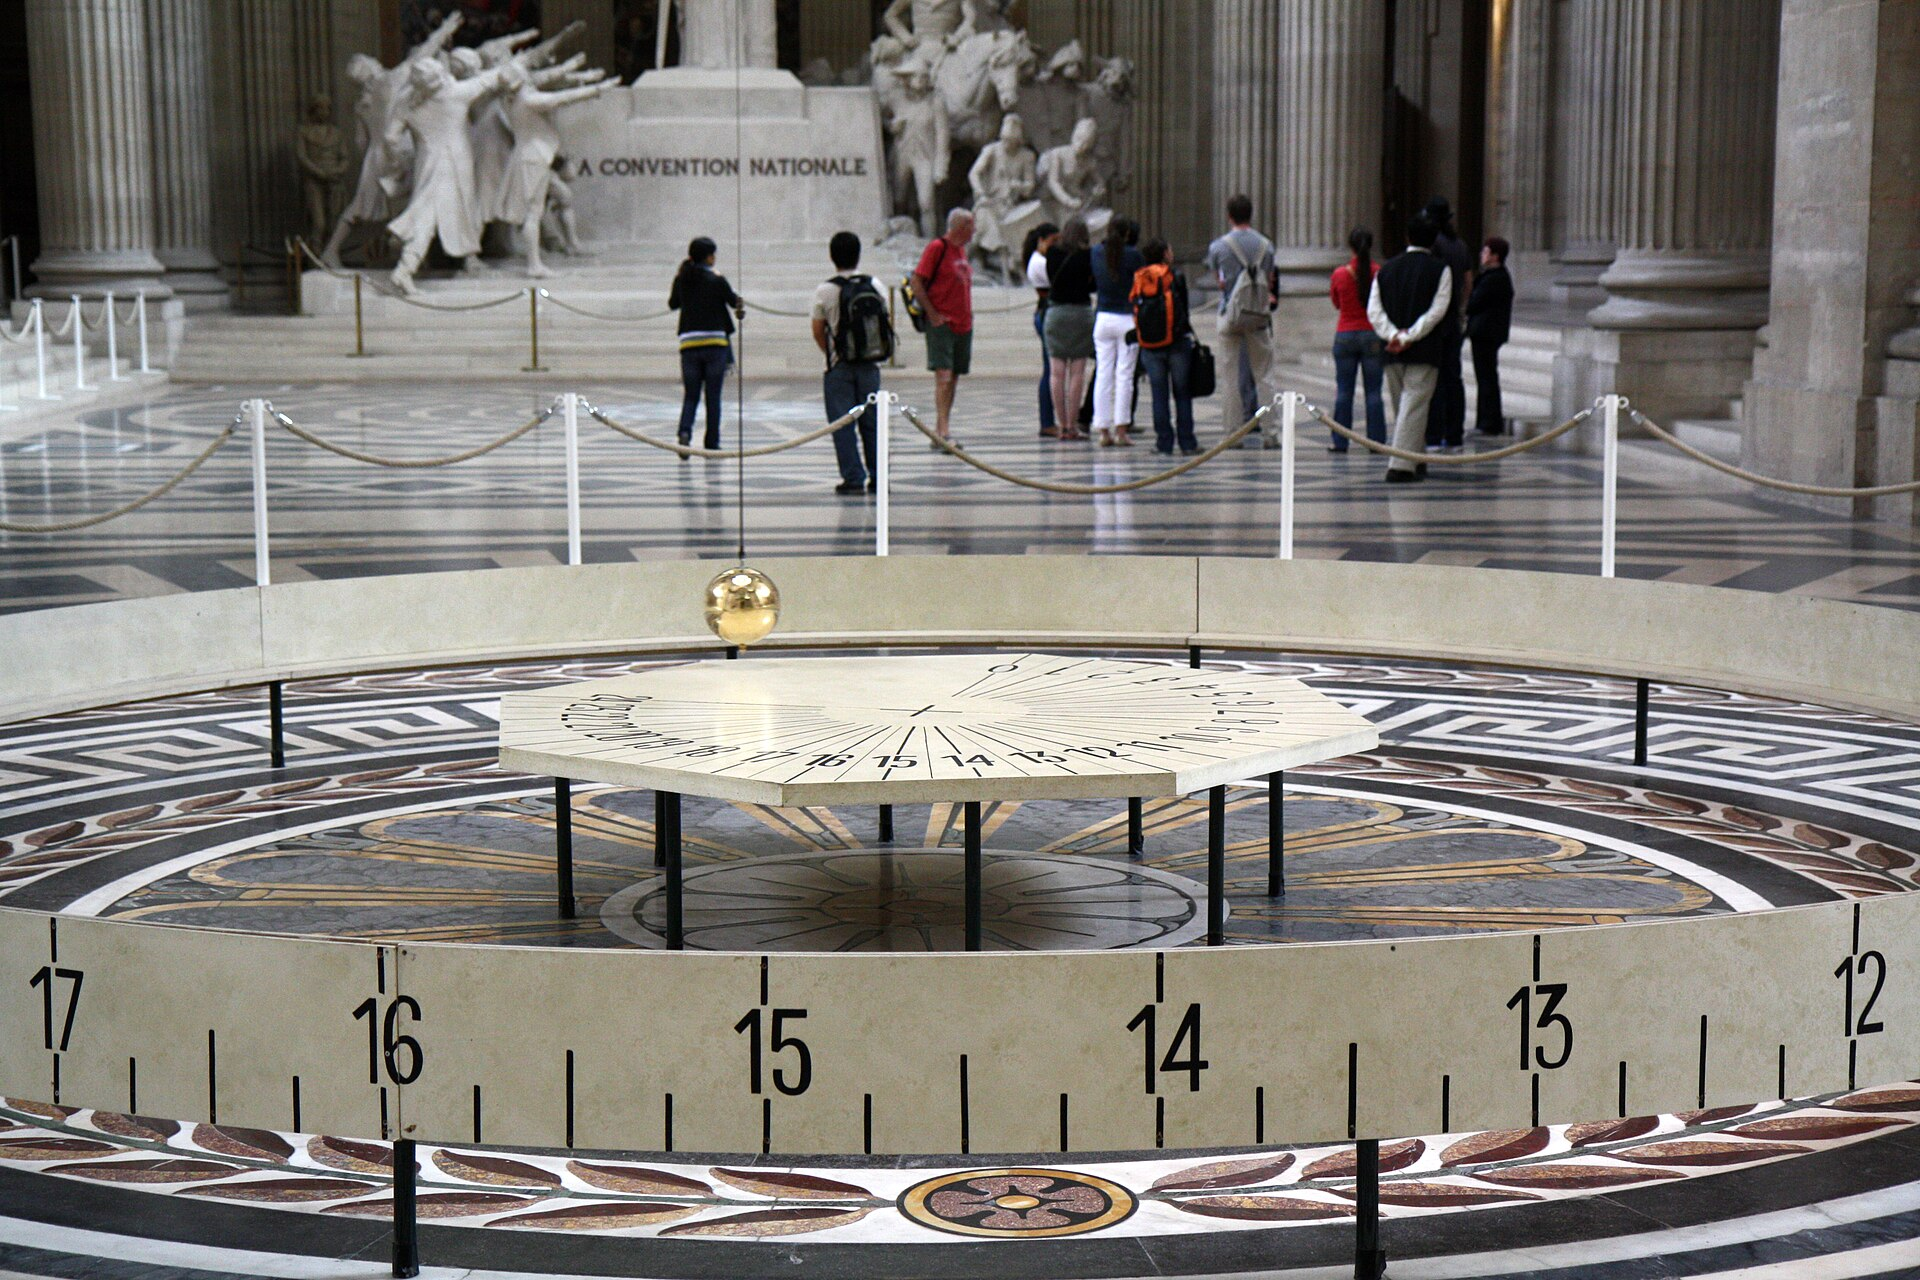
\includegraphics[width=0.6\linewidth]{images/book5/photo-foucault-pantheon.jpg}

{\small Le pendule de Foucault au Panthéon, à Paris. Des \omterm{def:b3:lagrangian-mechanics:coordinates}{coordonnées généralisées}, une \omterm{def:b3:lagrangian-mechanics:coordinates}{contrainte} et un référentiel qui tourne lentement~: la rotation de la salle apparaît dans les équations du mouvement --- et la dérive du plan d'oscillation permet à un sous-sol de mesurer la rotation de la Terre. Photographie~: Olga Khomitsevich, CC~BY~2.0.}
\end{omfigure}

\section{Problème~: le balai qui tient à l'envers}

\begin{problem}[{Problème du week-end --- le pendule inversé de Kapitza}]\label{pb:b3:lagrangian-mechanics:1}
Un pendule rigide peut tenir en équilibre stable \emph{au-dessus} de
son pivot si l'on secoue ce pivot de haut en bas assez vite --- une
découverte analysée par Kapitza en 1951, assez frappante pour
ressembler à un tour de prestidigitation, et le principe par lequel des
champs électriques oscillants piègent des ions uniques. Nous modélisons
le pendule par une masse ponctuelle $m$ au bout d'une tige rigide sans
masse de longueur $\ell = \qty{40}{cm}$~; $\theta$ est l'angle compté
depuis la verticale \emph{descendante}~; $g = \qty{9.81}{m/s^2}$.

\medskip\noindent\textbf{Partie I --- Le pendule rigide.}
Le pivot est d'abord maintenu fixe.
\begin{enumerate}
  \item Écrire le \omterm{def:b3:lagrangian-mechanics:action}{lagrangien} et l'équation du mouvement.
  \item Donner la fréquence $f_0$ des \omterm{prop:b3:lagrangian-mechanics:modes}{petites oscillations} autour de $\theta =
        0$, et sa valeur.
  \item Montrer qu'ici $h = E$, et utiliser sa conservation pour
        trouver la vitesse minimale de lancement de la masse, en bas,
        qui la mène jusqu'au sommet.
  \item Linéariser l'équation près de $\theta = \pi$ (poser $\theta = \pi +
        \epsilon$) et montrer que $\ddot\epsilon = +(g/\ell)\epsilon$~:
        à quelle vitesse un millidegré initial d'inclinaison croît-il~?
        Donner le temps qu'il met à croître d'un facteur $e$.
  \item Un balai en équilibre sur le bout du doigt tombe en une seconde
        environ, et pourtant ne tient jamais seul~: dites en une phrase
        ce que l'équation linéarisée affirme de l'équilibre $\theta = \pi$.
\end{enumerate}

\medskip\noindent\textbf{Partie II --- On secoue le pivot.}
Le pivot oscille maintenant verticalement, sa hauteur étant $y_{\text{s}}(t) =
a\cos\Omega t$ avec $a = \qty{2.0}{cm}$ et $\Omega$ réglable.
\begin{enumerate}[resume]
  \item Écrire les coordonnées de la masse et montrer que
        $\vect v^{\,2} = \ell^2\dot\theta^2 -
        2a\Omega\ell\sin(\Omega t)\sin\theta\,\dot\theta +
        a^2\Omega^2\sin^2\Omega t$.
  \item Montrer que deux \omterm{def:b3:lagrangian-mechanics:action}{lagrangiens} différant d'une dérivée totale en
        temps $\dd F(q,t)/\dd t$ donnent les mêmes \omterm{thm:b3:lagrangian-mechanics:euler-lagrange}{équations
        d'Euler--Lagrange}.
  \item Utiliser cette liberté pour ramener le \omterm{def:b3:lagrangian-mechanics:action}{lagrangien} à $L = \tfrac12 m
        \ell^2\dot\theta^2 - ma\Omega^2\ell\cos(\Omega t)\cos\theta +
        mg\ell\cos\theta$. (Indication~: le terme
        $\sin(\Omega t)\sin\theta\,\dot\theta$ se combine à un terme en
        $\cos(\Omega t)\cos\theta$ pour former une dérivée totale~; les
        termes ne dépendant que de $t$ peuvent être abandonnés.)
  \item Obtenir l'équation du mouvement
        \[
        \ddot\theta = -\frac{g}{\ell}\sin\theta
         + \frac{a\Omega^2}{\ell}\cos(\Omega t)\sin\theta .
        \]
        Interpréter le second terme comme le remplacement du poids par $g +
        \ddot y_{\text{s}}$~: le pendule vit dans un ascenseur.
  \item La \omterm{prop:b3:lagrangian-mechanics:energy}{fonction énergie} $h$ est-elle encore conservée~? Et
        l'énergie~? Qu'est-ce qui injecte et retire de l'énergie~?
  \item Dans le régime de Kapitza, $a \ll \ell$ et $\Omega \gg \omega_0 =
        \sqrt{g/\ell}$~: le vérifier pour $a = \qty{2}{cm}$, $\ell =
        \qty{40}{cm}$, $\Omega/2\pi = \qty{40}{Hz}$, et expliquer
        physiquement pourquoi la masse ne peut alors pas suivre
        l'excitation.
\end{enumerate}

\medskip\noindent\textbf{Partie III --- Séparer le rapide du lent.}
Cherchons le mouvement sous la forme $\theta(t) = \Theta(t) + \xi(t)$~:
une dérive lente $\Theta$ plus une petite ondulation $\xi$ à la fréquence d'excitation.
\begin{enumerate}[resume]
  \item En ne gardant que le plus grand terme de chaque membre, montrer
        que l'ondulation obéit à $\ddot\xi \approx +(a\Omega^2/\ell)\cos(\Omega t)
        \sin\Theta$, avec $\Theta$ gelé à l'échelle de temps de
        l'excitation.
  \item En déduire $\xi(t) = -(a/\ell)\cos(\Omega t)\sin\Theta$, et
        vérifier que son amplitude est petite, de l'ordre de $a/\ell$.
  \item Développer $\sin\theta = \sin(\Theta + \xi)$ au premier ordre en
        $\xi$ et reporter dans l'équation du mouvement.
  \item Moyenner sur une période d'excitation, $\Theta$ étant maintenu
        fixe~: à l'aide de $\langle\cos\Omega t\rangle = 0$ et de
        $\langle\cos^2\Omega t\rangle = \tfrac12$, montrer que
        \[
        \ddot\Theta = -\frac{g}{\ell}\sin\Theta
         - \frac{a^2\Omega^2}{2\ell^2}\sin\Theta\cos\Theta .
        \]
  \item Montrer que c'est un mouvement dans le potentiel effectif
        \[
        U_{\text{eff}}(\Theta) = mg\ell\Big({-\cos\Theta}
         + \frac{a^2\Omega^2}{4g\ell}\sin^2\Theta\Big) .
        \]
  \item Comparer avec la perle sur le cerceau tournant
        (\cref{ex:b3:lagrangian-mechanics:hoop})~: mêmes
        mathématiques, signe opposé du terme nouveau --- que fait
        l'excitation à l'équilibre du \emph{bas} que la rotation ne
        faisait pas~?
  \item Tracer $U_{\text{eff}}$ pour une excitation lente puis rapide,
        et décrire chaque équilibre et sa stabilité dans les deux cas.
\end{enumerate}

\medskip\noindent\textbf{Partie IV --- Le balai se dresse.}
\begin{enumerate}[resume]
  \item En développant $U_{\text{eff}}$ près de $\Theta = \pi$, montrer
        que la position inversée est stable exactement lorsque
        \[
        a^2\Omega^2 > 2g\ell .
        \]
  \item Calculer la fréquence critique d'excitation $f_{\text{c}} =
        \Omega_{\text{c}}/2\pi$ pour notre pendule, ainsi que la
        vitesse maximale du pivot $a\Omega_{\text{c}}$ et
        l'accélération $a\Omega_{\text{c}}^2$ (en unités de $g$)
        qu'elle exige.
  \item À $\Omega = 2\Omega_{\text{c}}$, trouver la fréquence du
        balancement lent du pendule dressé autour de $\Theta = \pi$, et
        sa valeur~; vérifier qu'elle est bien lente devant
        l'excitation.
  \item Toujours à $\Omega = 2\Omega_{\text{c}}$, quelle est
        l'amplitude $\xi$ de l'ondulation pour $\Theta$ légèrement
        écarté de $\pi$, en degrés, pour $a/\ell = 0.05$~? Une
        photographie trahirait-elle le tour~?
  \item De combien le balai peut-il pencher hors de la verticale et
        revenir tout de même~? Montrer que le puits du pendule dressé
        s'étend sur $|\Theta - \pi| <
        \arccos(2g\ell/a^2\Omega^2)$, et l'évaluer à $\Omega =
        2\Omega_{\text{c}}$.
  \item Un jongleur qui tient un balai en équilibre sur un doigt
        immobile y parvient aussi --- par quel mécanisme entièrement
        différent~? Nommer la propriété du pendule de Kapitza qui ne
        demande aucune rétroaction.
  \item Résumer le résultat nommé~: un pivot secoué à \qty{45}{Hz} avec
        une amplitude de \qty{2}{cm} --- deux fois la fréquence
        critique --- maintient un pendule de \qty{40}{cm} la tête en
        bas, dans un puits atteignant quelque $75^\circ$ depuis la
        verticale, oscillant doucement à environ \qty{1.4}{Hz}. Où, en
        physique, ce même piégeage moyenné sert-il à retenir une
        particule chargée unique~?
\end{enumerate}
\end{problem}
